\section{Behavior and Verification of Correctness}
In this section, we will explain how the algorithm behaves in cases where, due to the problem of the experimenter's regress\footnote{In order to judge whether our algorithm is correct we must rely on a theoretical correct solution, and to produce such a solution we would need an algorithm that is known to be correct.}, we were unable to formally verify our algorithm's output. We have instead tested the output around edge cases, and argued why the output is correct. We use a 6 by 6 grid:
\begin{figure}[H]
    \centering
    \caption{Reference grid for tests}
    \label{gridTest}
    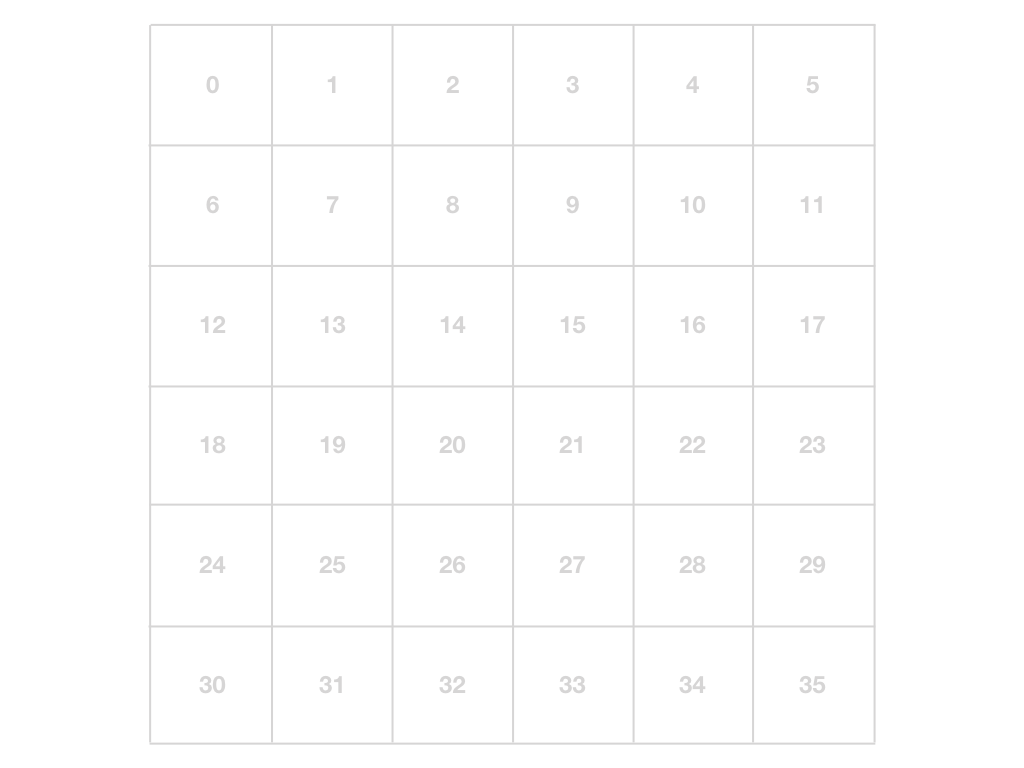
\includegraphics[width=0.5\textwidth]{figures/test_grid.png}
\end{figure}

\subsection*{Vertical lines}
Running the algorithm for a single line with an angle of 0, passing through the center of the grid, we get the following output:
\begin{table}[H]
    \centering
    \caption{Test result - angle 0}
    \begin{tabular}{llllllllllll}
    Index  & 33 & 27 & 21 & 15 & 9 & 3 & -1 & -1 & -1 & -1 & -1 \\
    Length & 1  & 1  & 1  & 1  & 1 & 1 & -1 & -1 & -1 & -1 & -1
    \end{tabular}
\end{table}
An index and length of $-1$ is just the result of the padding that ensures that all arrays are of equal length, and can thus be ignored. Visualized on the grid, we see that the line is indeed vertical and correctly located in the center of the grid:
\begin{figure}[H]
    \centering
    \caption{Test - 0 angle}
    \label{test0}
    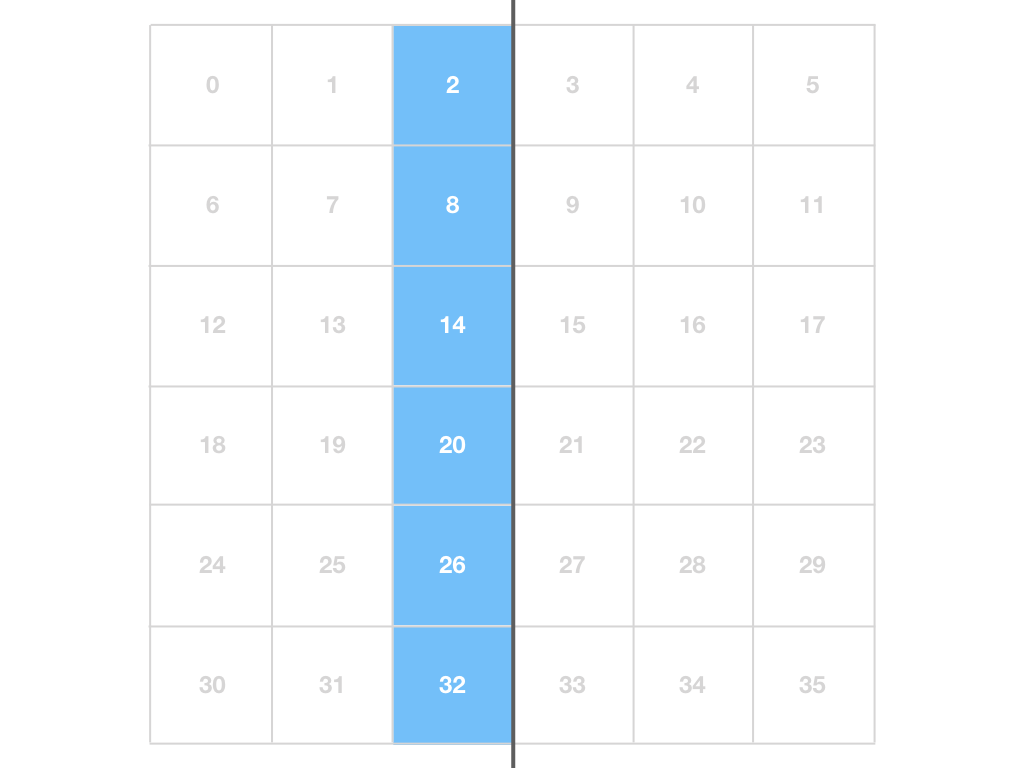
\includegraphics[width=0.5\textwidth]{figures/test_0.png}
\end{figure}
We note that every length is reported as exactly $1$, in accordance with our expectations, since $1$ represents the standardized width and height of a pixel.
Since the line passes exactly through the center of the grid, a choice has to be made as to which pixel column to report the line as passing through. As evident by figure \ref{test0}, we have arbitrarily chosen the report the pixel column to the left.\\

Changing the angle to 1 degree, we get:
\begin{table}[H]
    \centering
    \caption{Test result - 0 degree angle}
    \begin{tabular}{llllllllllll}
    Index  & 32 & 26 & 20 & 15 & 9 & 3 & -1 & -1 & -1 & -1 & -1 \\
    Length & 1.00015  & 1.00015  & 1.00015  & 1.00015  & 1.00015 & 1.00015 & -1 & -1 & -1 & -1 & -1
    \end{tabular}
\end{table}
As expected, the line has now shifted as seen on figure \ref{test1}, and the lengths are now slightly larger than $1$, reflecting the fact the the line passes through each pixel at an angle. 
\begin{figure}[H]
    \centering
    \caption{Test - 1 degree angle}
    \label{test1}
    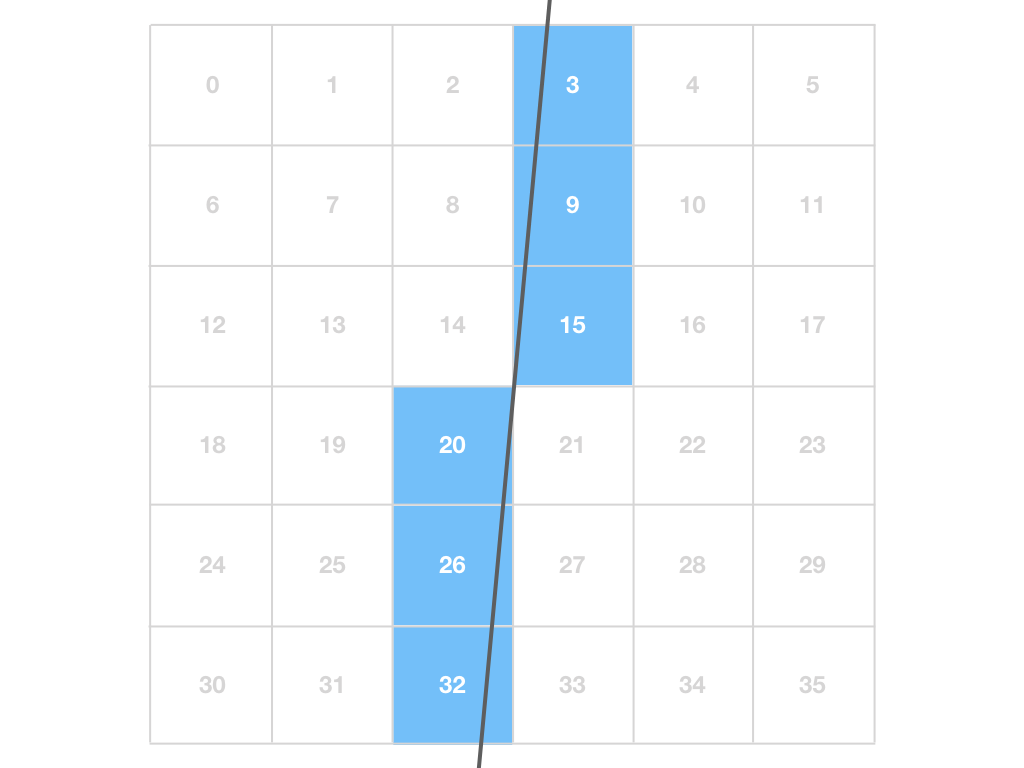
\includegraphics[width=0.5\textwidth]{figures/test_1.png}
\end{figure}

\subsection*{Horizontal lines}
Moving on to horizontal and near-horizontal lines we get the following output for 90 degrees:
\begin{table}[H]
    \centering
    \caption{Test result - angles 89, 90 and 91}
    \begin{tabular}{llllllllllll}
    Index  & 12 & 13 & 14 & 15 & 16 & 17 & -1 & -1 & -1 & -1 & -1 \\
    Length & 1  & 1  & 1  & 1  & 1 & 1 & -1 & -1 & -1 & -1 & -1 
    \end{tabular}
\end{table}
Similar to the vertical lines, we see lengths of $1$ and a perfectly horizontal line, situated in the pixel row directly above the center:
\begin{figure}[H]
    \centering
    \caption{Test - 90 degree angle}
    \label{test90}
    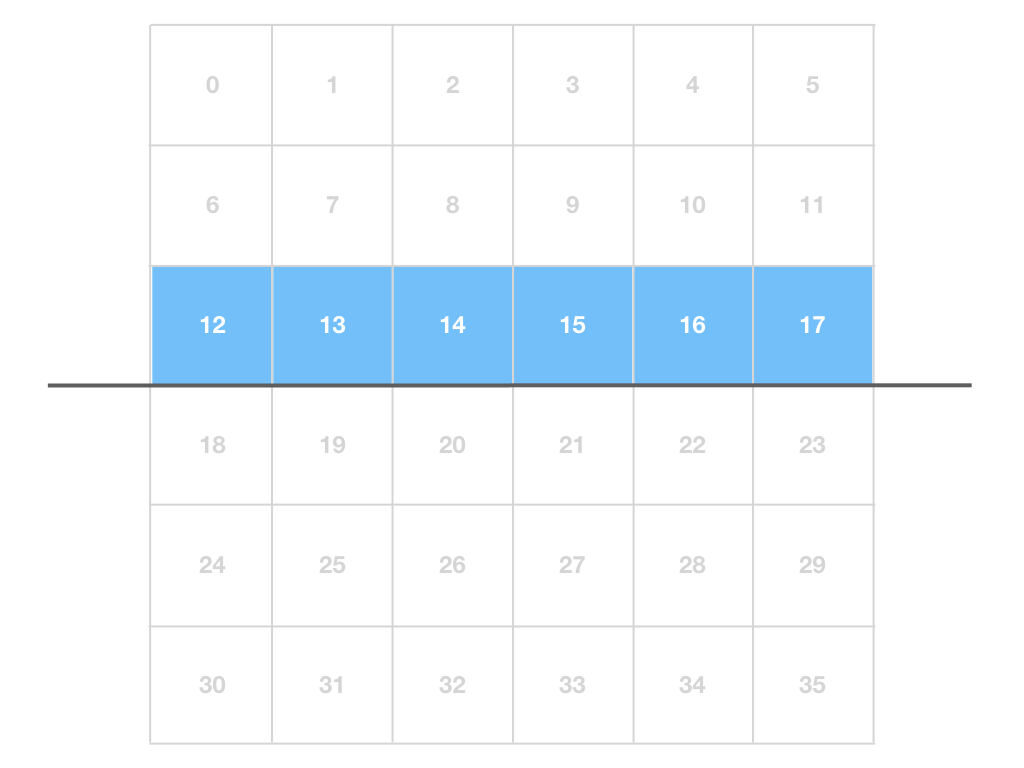
\includegraphics[width=0.5\textwidth]{figures/test_90.png}
\end{figure}
Visualized on a grid, testing 89 and 91 degree angles yields the following line: 
\begin{figure}[H]
    \centering
    \begin{minipage}[b]{0.49\textwidth}
        \centering
        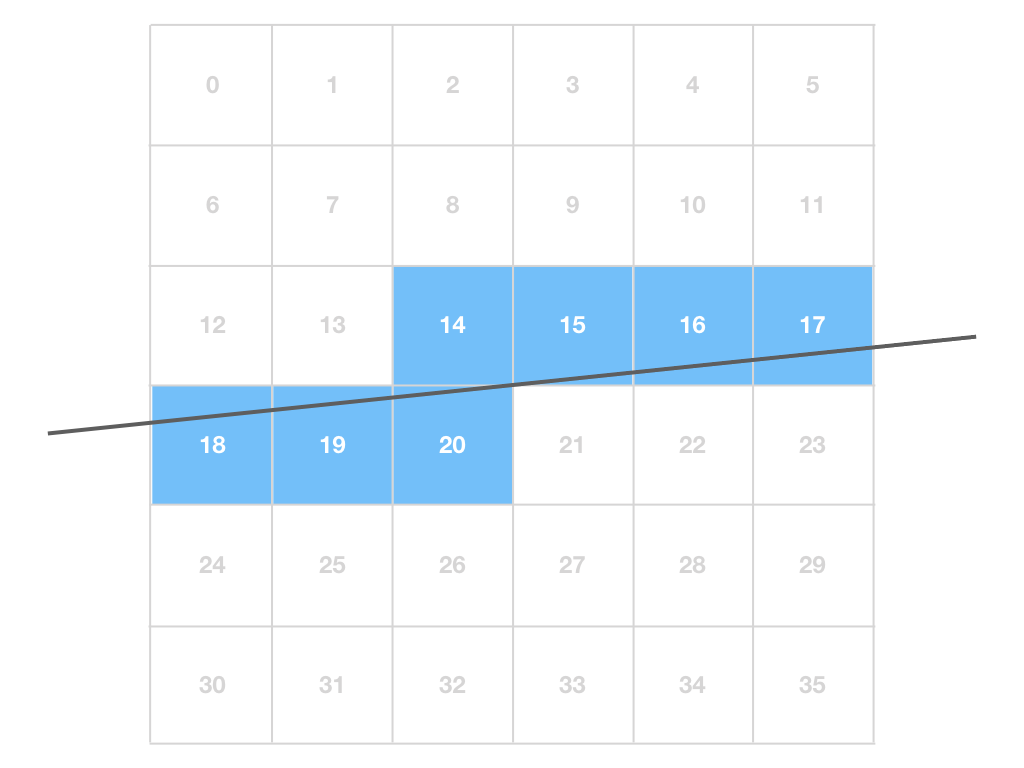
\includegraphics[width=0.49\textwidth]{figures/test_89.png}
        \caption{Test - 89 degree angle}\label{test89}
    \end{minipage}
    \begin{minipage}[b]{0.49\textwidth}
        \centering
        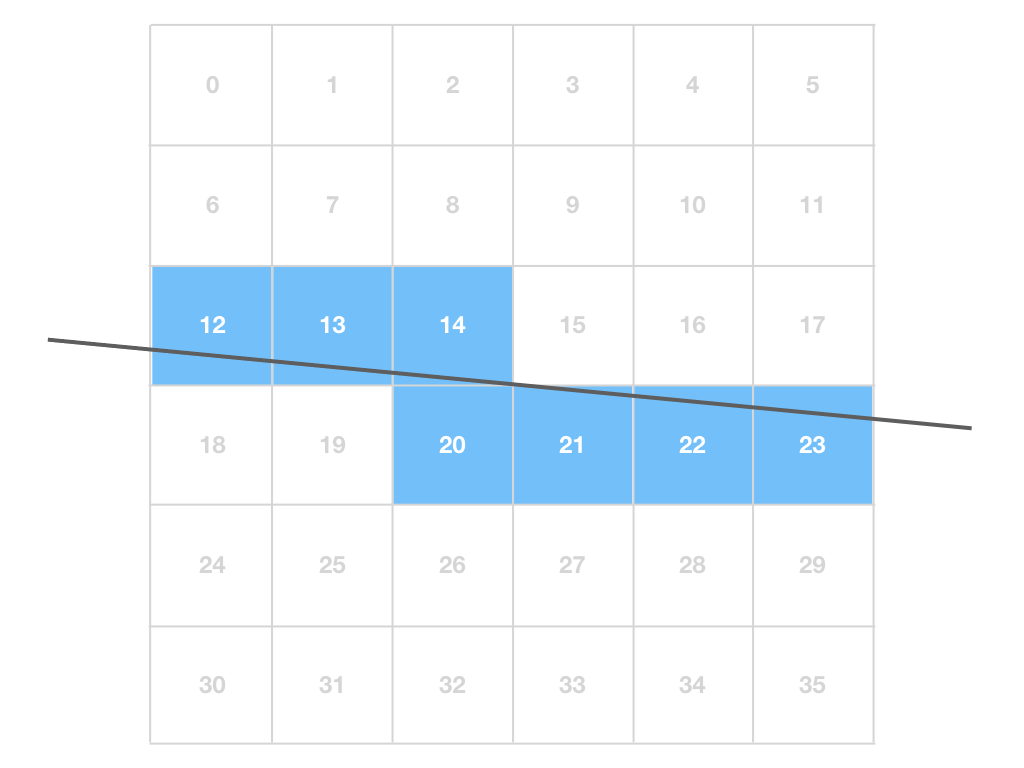
\includegraphics[width=0.49\textwidth]{figures/test_91.png}
        \caption{Test - 91 degree angle}\label{test91}
    \end{minipage}
\end{figure}
We see that a small error has crept in, since pixel $14$ and $20$ are being reported as having part of the lines passing through them, even though this should not be the case. Looking at the actually lengths attributed to these pixels, reveals that these are practically zero, i.e. $0.00001$. This can occur in situations when the line passes exactly through a grid coordinate, such as $(0,0)$, in which case, even a small floating point error, can result in the algorithm thinking that the line passes ever so slightly through an adjacent pixel. Since this erroneous pixel will always be adjacent to a true pixel, and since the erroneous pixel is ascribed a very small length, this is deemed to not be a problem.

Similar testing has been carried out for other interesting angles, such as the area around $45$, $135$ and $180$ degrees, but for the sake of keeping this section short, we will not discuss the results in depth, and instead simply note that the algorithm behaves as expected in these cases. 
